\section{Anti-Serialization} \label{sec:as}
In this section we will describe a set of transformation rules known as Anti-Serializations. In \cref{fig:trivial-example} all items made according to the three recipes in \cref{fig:toy-recipes} will have to pass through modules, which do not work on them. We would like to minimize this as to reduce the total length that each item must be transported, in addition to combating bottlenecks in the line. Thus it would be beneficial if items could bypass modules that do not work on them. We get around this by branching out production on more lines, where items only go through modules that work on them. 

\subsection{$AS_0$: Branch Between Common Modules}
We start by defining the most common type of anti-serialization with the $AS_0$ transformation rule given in \cref{def:as0}. Informally the rule states that if we have a set of modules $B_{r,s,e}$, which works the recipe $r \in R$ exclusively, lying between the modules $s$ and $e$ on $\Gamma_0$ then we may branch out all modules in $B_{r,s,e}$ to form a new line. This new line is connected to $\Gamma_0$ at $s$ and $e$. We will explain this more in depth, by going over the sets brough up in the rule. 

\begin{definition}[htb]
\runatt{AS}{0}
    \infrule
        {0 < |B_{r,s,e}| \land  s <_k e}
        {(R,M,\Gamma, \Gamma_0, AW, Start, End) \rightarrow_{AS}
        (R,M,\Gamma', \Gamma_0', AW, Start', End') } \\
        Where: \\
        $r \in R$ \\
		$s,e \in K_{\Gamma_0,r}$\\		
		$\Gamma_0' = (Pre_s \cup \{s\}  \cup A_{r,s,e} \cup \{e\} \cup Pos_e, \prec)$ \\     
        $\Gamma' = \Gamma \cup B_{r,s,e} $ \\
		$Start' = Start \cup \{(B_{r,s,e}, s)\}$ \\
		$End' = End \cup \{(B_{r,s,e}, e)\}$

\caption{Formal definition of the $AS_0$ transformation rule}
\label{def:as0}
\end{definition}

We initially define a special set on $r$, $\bar{r}$, which contains all types of work which are not unique to $r$:
\[\bar{r} = \bigcup_{r' \in R}r', \texttt{ if } r' \neq r\]

Next we define, what we refer to as common modules. These are modules in $\Gamma_0$, which $r$ needs to use along with at least some other recipe. These are important to identify, as they may not be branched out, since that would make them inaccessible to the other recipes than $r$. Given $r$ and $\Gamma_0$ we define the set of common modules $K_{\Gamma_0,r}$ as follows:

\[K_{\Gamma_0 ,r} = \{m | m \in \Gamma_0  \land \exists \rho \in AW(m),\, \{\rho\} \subseteq r \land \{\rho\} \subseteq \bar{r} \land r \in R\}\]

From this set we can then define $\alpha_{\Gamma_0 ,r}$, which is the set of modules in $\Gamma_0$ which are not used by $r$: 

\[\alpha_{\Gamma_0 ,r}  = \{m |m \in \Gamma_0 \land \forall \rho \in AW(m),\, \{\rho\} \nsubseteq r \land r \in R\}\]

Along with $\beta_{\Gamma_0 ,r}$, which is the set of modules in $\Gamma_0$ used only by $r$:

\[\beta_{\Gamma_0 ,r}  = \{m  | m \in \Gamma_0 \land \forall \rho \in AW(m),\, \{\rho\} \subseteq r \land \{\rho\} \nsubseteq \bar{r} \land r \in R\}\]

Next we define the binary relation relation $<_K$ as:
\[a <_K b = \left\{\begin{matrix}
tt \texttt{ if } a,b,c \in K_{\Gamma_0 ,r} \land a \prec b \land \lnot (a \prec c \land c \prec b) \\ \texttt{else } ff
\end{matrix}\right.\]

We also define a total order of all modules in between two modules, $s$ and $e$, in some line $\gamma \in \Gamma$:

\[M_{s,e} = (\{m | m \in \gamma \land \gamma \in \Gamma \land s \prec m \land m \prec e\}, \prec)\]

We can now define the total order of all modules appearing between $s$ and $e$, which are not used to work $r$, $A_{r,s,e}$ as follows: 

\[A_{r,s,e} = (\{m |m \in M_{s,e} \land m \in \alpha\}, \prec)\]

Similarly we can define the total order $B_{r,s,e}$, which contains all modules that appear between $s$ and $e$ which work exclusively on $r$

\[B_{r,s,e} = (\{m |m \in M_{s,e} \land m \in \beta\}, \prec)\]

We define $Pre_{s}$ which is the set of all modules that come before a module $s$ in line $\gamma \in \Gamma$:
\[Pre_{s} = (\{m | m \in \gamma \land \gamma \in \Gamma \land m \prec s\}, \prec)\]

And lastly we define $Pos_{e}$ which is the set of all modules that come after a module $e$  in line $\gamma \in \Gamma$:
\[Pos_{e} = (\{m | m \in \gamma \land \gamma \in \Gamma \land e \prec  m \}, \prec)\]

Having defined these sets the rule in \cref{def:as0}, shows that in the case where $|B_{r,s,e}| > 0 \land s <_K e$ then we may update $\Gamma$ with a new lines defined by the total order $B_{r,s,e}$ in addition to an update of $\Gamma_0$, which removes $B_{r,s,e}$ from the line. This describes a branch out from $\Gamma_0'$, which exclusively works upon $r$ before rejoining with the old line.   

While this rule is formally sound, it can be difficult to read. As such we have tried to illustrate the transformation from configuration to configuration visually in \cref{fig:as0}. This visualization uses a homemade notation. Square boxes refer to individual modules. Boxes with rounded corners are total orders of sets of modules. A graphical line of boxes flowing from left to right is a line in $\Gamma$ ordered as shown. If a module $s$ and a line $\gamma$ are connected by a vertical upward going edge, then $Start$ contains the ordered pair $(\gamma ,s)$. At the same time, if the edge goes downwards from a line $\gamma$ to a module $e$, then $End$ contains the ordered pair $(\gamma ,e)$.


\begin{figure}[H]
\centering
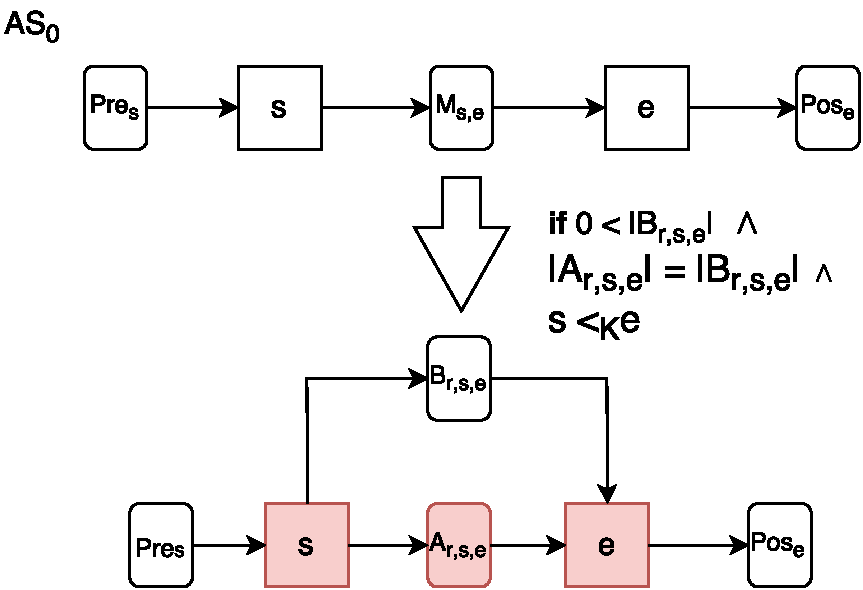
\includegraphics[width=\textwidth]{as0.pdf}
\caption{A visual representation of the $AS_0$ transformation rule}
\label{fig:as0}
\end{figure}

For the rest of this chapter, we will use these visualization to explain our transformation rules, instead of setting up transition rules. If any new derived sets are shown in a new transformation rule, we will describe them as well. Note that while we always show new lines appearing above an old line, a new line may be placed at either side in either of the rules described in this chapter.  

In the rest of this section we will describe two special cases known as $AS_1$, branch in, and $AS_2$, branch out. 

\subsection{$AS_1$: Branch In}\label{sssec:bi}
It may be that we have modules that precede the first module of $K_{\Gamma_0 ,r}$ that we would like to branch out, but can not with the rule described in \cref{def:as0}, as it requires two distinct $K_{\Gamma_0 ,r}$ modules. In this case, we describe the transformation rule $AS_1$, which can be seen in \cref{fig:as1}.

\begin{figure}[H]
	\centering
	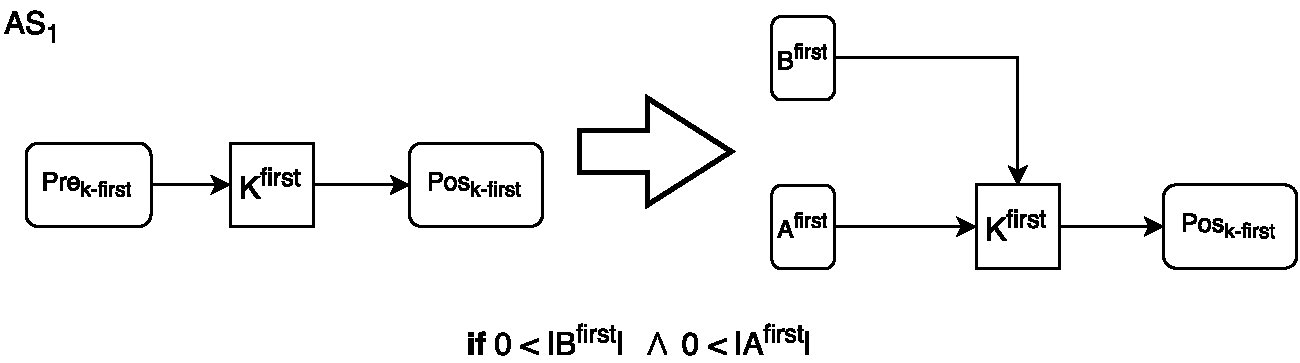
\includegraphics[width=\textwidth]{as1.pdf}
	\caption{A visual representation of the $AS_1$ transformation rule. This is used for the case where we which to branch out modules prior to the first element of $K_{\Gamma_0 ,r}$}
	\label{fig:as1}
\end{figure}


 We define the first module in $K_{\Gamma_0 ,r}$ as:

\[K_{\Gamma_0 ,r}^{first} = m \texttt{ where } \forall m' \in K_{\Gamma_0 ,r} \land m \neq m',\, m \prec m' \] 

Similarly for the $AS_0$ transformation rule, we define two total orderings. $A_{\Gamma_0 ,r}^{first}$ that describes all modules before $K_{\Gamma_0 ,r}^{first}$ which do not work on $r$. And $B_{\Gamma_0 ,r}^{first}$ which describes all modules before $K_{\Gamma_0 ,r}^{first}$ which exclusively works on $r$.

\[ A_{\Gamma_0 ,r}^{first} = (\{m | m \in \alpha_{\gamma ,r}  \land m \in Pre_{K_{\Gamma_0 ,r}^{first}} \}, \prec) \]

\[ B_{\Gamma_0 ,r}^{first} = (\{m | m \in \beta_{\gamma ,r}  \land m \in Pre_{K_{\Gamma_0 ,r}^{first}} \}, \prec) \]

We also again use the $Pre_s$ and $Pos_e$ sets here, but used on $K_{\Gamma_0 ,r}^{first}$ instead of $s$ and $e$ as in the case of the previous rule.
  

\subsection{$AS_2$: Branch Out}
Similarly to $AS_1$ we have the case, where the last element in $K_{\gamma ,r}$, is proceeded by a set of modules that we would like to branch out. For this we describe the transformation rule $AS_2$, which can be seen in \cref{fig:as2}.

\begin{figure}[H]
	\centering
	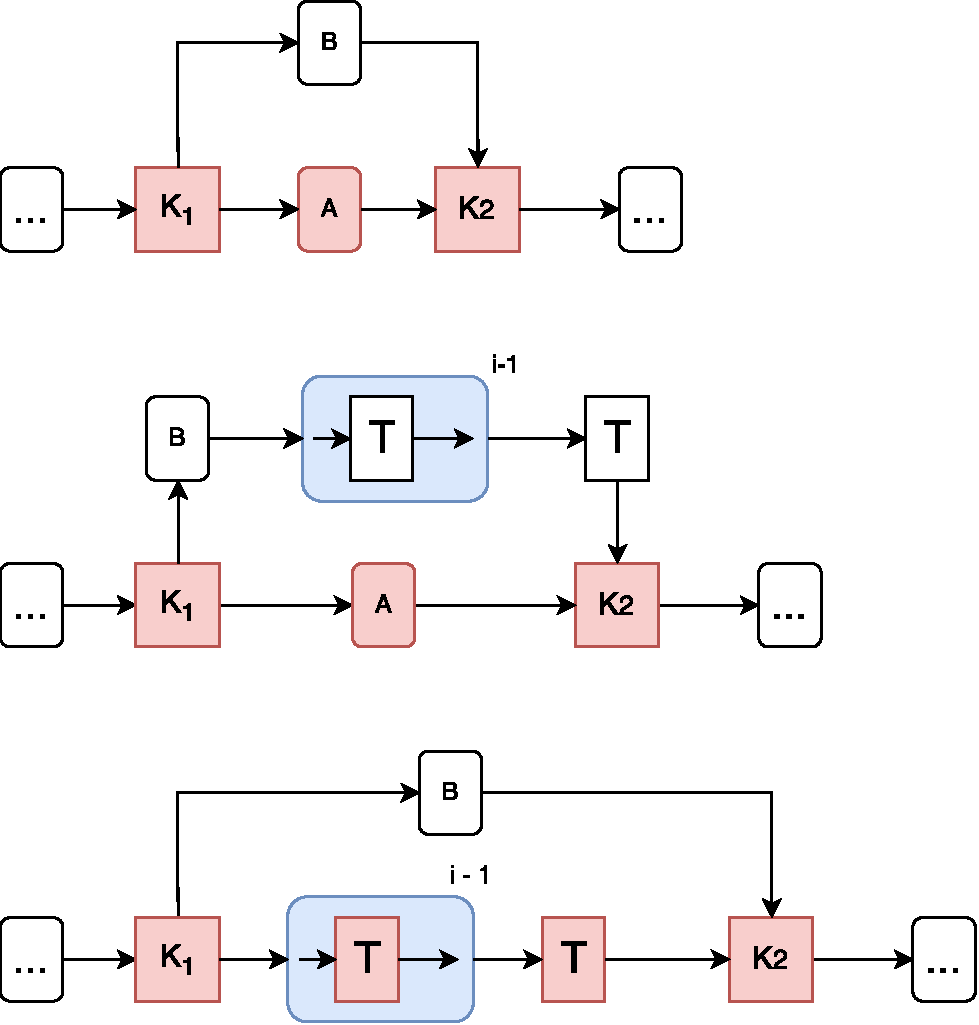
\includegraphics[width=\textwidth]{as2.pdf}
	\caption{A visual representation of the $AS_2$ transformation rule. This is used for the case where we which to branch out modules proceeding the last element of $K_{\Gamma_0 ,r}$}
	\label{fig:as2}
\end{figure}


We define the last module in $K_{\Gamma_0 ,r}$ as:

\[K_{\Gamma_0 ,r}^{last} = m \texttt{ where } \forall m' \in K_{\Gamma_0 ,r} \land m \neq m',\, m' \prec m \] 


Again we also define two total orders. $A_{\Gamma_0 ,r}^{last}$ that describes all modules after $K_{\Gamma_0 ,r}^{last}$ which do not perform any work on $r$. And $B_{\Gamma_0 ,r}^{last}$ which describes all modules after $K_{\Gamma_0 ,r}^{last}$, which exclusively works on $r$.


\[ A_{\Gamma_0 ,r}^{last} = \{m | m \in \alpha_{\gamma ,r}  \land m \in Pos_{K_{\Gamma_0 ,r}^{last}} \} \]

\[B_{\Gamma_0 ,r}^{last} = \{m | m \in \beta_{\gamma ,r}  \land m \in Pos_{K_{\Gamma_0 ,r}^{last}} \}\]

